\documentclass[oneside]{book}
\usepackage{../Style/Master}
\usepackage{../Style/boxes}
\usepackage{../Style/Env}
\usepackage{../Style/DefNoteFact}
\usepackage{../Style/QnsProof}
\usepackage{../Style/Thms}
\usepackage{newpxtext, eulerpx}
\usepackage{bbding}
\usepackage{pgf-interference}
\begin{document}
A ``\(\circ\)''  denotes a point outside of accuracy/precision/safety precautions.
\begin{longtable}{M{0.1\textwidth}m{0.4\textwidth}m{0.4\textwidth}}
    \toprule
    Topic & \centering Accuracy/Precision & \centering Safety
    \tabularnewline\midrule
    General &
    \begin{itemize}
        \item[\textcolor{green!70!black}{\checkmark}] Always take preliminary readings.
        \item[\textcolor{green!70!black}{\checkmark}] Measure \(t\) thrice and take the average.
        \item[\textcolor{green!70!black}{\checkmark}] Remove all other sources of \rule{1cm}{0.01mm} (sound/light/etc) before conducting the experiment, to reduce systematic/random error. \hyperlink{error:other-sources-of-alternating-magnetic-fields}{(circuits e.g.)} \hyperlink{error:other-sources-of-sound}{(sound e.g.)}
    \end{itemize}
    &
    \tabularnewline\midrule
    Nuclear & 
    \begin{itemize}
        \item[\textcolor{green!70!black}{\checkmark}] Preliminary readings. E.g. Determine the range of distances \(d\) and thicknesses \(t\) of front plates that will give a measurable difference in the count rate. 
        \item[\textcolor{green!70!black}{\checkmark}] Repeat the measurements for \(C_b\) and \(C_T\) thrice and take the average.
        \item[\textcolor{green!70!black}{\checkmark}] Measure the background count rate \(C_b\) and subtract it from the total count rate \(C_T\), to obtain the count rate \(C=C_T-C_b\) of the sample.   
    \end{itemize}
    &
    \begin{itemize}
        \item[\textcolor{green!70!black}{\checkmark}] The source is handled with a pair of tongs, to prevent contact with the radioactive material.
        \item[\textcolor{green!70!black}{\checkmark}] The source is stored in a lead lined box when not in use, to prevent contact with the radioactive material.
        \item[\textcolor{green!70!black}{\checkmark}] Cordon off the area with tape and put up a warning sign, to prevent others from being exposed to radioactive material. 
        \item[\textcolor{red}{\(\times\)}] Avoid pointing the source at people.
        \item[\textcolor{red}{\(\times\)}] Do not look directly at the source.
        \item[\textcolor{red}{\(\times\)}] Protective clothing, lead suits, lead gloves, goggles.   
    \end{itemize}
    \tabularnewline\midrule
    Thermal & &
    \begin{itemize}
        \item[\textcolor{green!70!black}{\checkmark}] Wear heat insulating gloves.
        \item[\textcolor{green!70!black}{\checkmark}] Avoid touching the hot objects.
    \end{itemize}
    \tabularnewline\midrule
    Waves &
    \begin{itemize}
        \item Sound
        \begin{itemize}
            \item[\textcolor{green!70!black}{\checkmark}] \hypertarget{error:other-sources-of-sound}{Conduct the experiment in a soundproofed room, to minimise random error due to environmental noise.}   
        \end{itemize} 
    \end{itemize}   
    &
    \begin{itemize}
        \item Light
        \begin{itemize}
            \item[\textcolor{green!70!black}{\checkmark}] Do not look directly at the light source, or point it directly at anyone.
            \item[\textcolor{green!70!black}{\checkmark}] Wear a pair of laser safety glasses (or shades for non-lasers) to protect the eyes.
            \item[\textcolor{green!70!black}{\checkmark}] Wear heat insulating gloves when moving the hot light source.  
        \end{itemize}
        \item Sound
        \begin{itemize}
            \item[\textcolor{green!70!black}{\checkmark}] Wear ear muffs to prevent hearing damage.
            \item[\textcolor{green!70!black}{\checkmark}] Switch on the sound source for a short period of time; turn it off when the apparatus is not in use.
        \end{itemize}
    \end{itemize}
    \tabularnewline\midrule
    Mechanics &
    \begin{itemize}
        \item[\textcolor{green!70!black}{\checkmark}] Explain clearly how to find the frequency of vibration \(f\). 
        
        Starting with the highest available frequency, the frequency of strobing is gradually reduced till the vibrating object appears stationary. Record the frequency of vibration \(f\) as the frequency of strobing.  
        \item[\textcolor{green!70!black}{\checkmark}] Explain clearly how to use a pair of photogates with an electronic timer to obtain the time taken \(t\).

        The object is projected so that it passes through both photogates. Record the times at which it passes through each gate as \(t_1\) and \(t_2\). Calculate the time taken \(t=t_2-t_1\).
        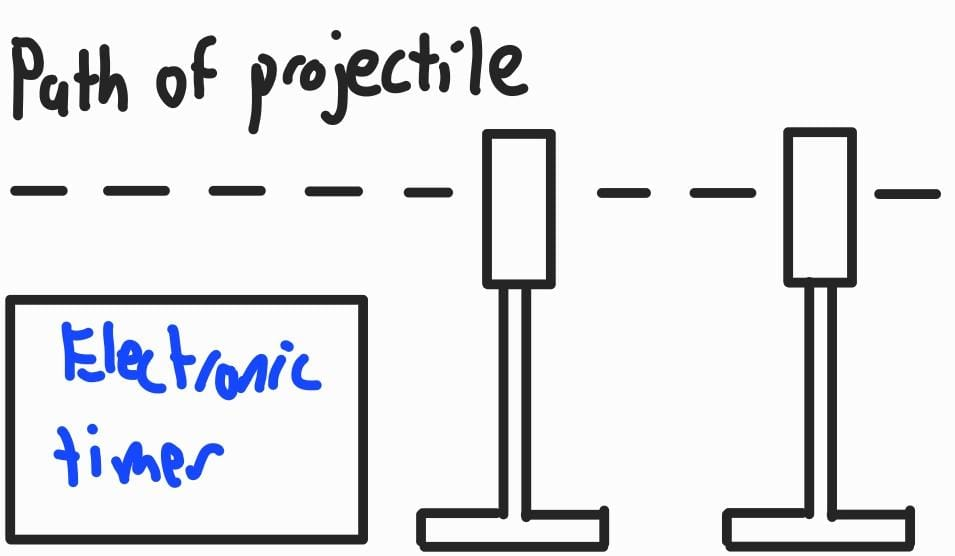
\includegraphics[width=\linewidth]{../images/electronic-timer-light-gates.jpg}
        When the distance between the gates is small, the average velocity\({}\approx{}\)instantaneous velocity.
    \end{itemize}
    & 
    \begin{itemize}
        \item Water/oil
        \begin{itemize}
            \item[\textcolor{green!70!black}{\checkmark}] Mop up any spillage of oil/water to avoid injuries due to falling.
        \end{itemize}
        \item Load
        \begin{itemize}
            \item[\textcolor{green!70!black}{\checkmark}] Wear safety boots to reduce possible injuries to your feet.
        \end{itemize}
        \item Moving parts
        \begin{itemize}
            \item[\textcolor{green!70!black}{\checkmark}] Avoid the moving blades of the fan using a safety screen. Switch off the fan when the apparatus is not in use. 
        \end{itemize}
        \item Glass
        \begin{itemize}
            \item[\textcolor{green!70!black}{\checkmark}] Wear thick safety googles and thick gloves to prevent injury when handling the glass.
        \end{itemize}
    \end{itemize}
    \tabularnewline\midrule
    \newpage\midrule
    E\&M &
    \begin{itemize}
        \item[\textcolor{green!70!black}{\checkmark}] Preliminary readings. E.g. Determine the range of frequencies \(f\) of e.m.f. and cross sectional area of the coil \(X\) that lead to a measurable range of induced e.m.f. \(\varepsilon\).
        \item[\textcolor{green!70!black}{\checkmark}] Use an iron core to increase the e.m.f. induced.
        \item[\textcolor{green!70!black}{\checkmark}] Detailed description on how to use the cathode ray oscilloscope (c.r.o.) to obtain raw data. E.g. 
        \begin{enumerate}
            \item Using the grid on the screen, measure the maximum vertical distance \(y\) occupied by a complete waveform. Multiply \(y\) by the scale indicated on the \(Y\)-gain to obtain the peak voltage \(V_0\).
            \item Using the grid on the screen, measure the horizontal distance \(x\) occupied by a complete waveform. Multiply \(x\) by the scale indicated on the time base to obtain the period \(T\).
        \end{enumerate}
        (The c.r.o. should be connected in parallel for the above.)
        \item[\textcolor{green!70!black}{\checkmark}] \hypertarget{error:other-sources-of-alternating-magnetic-fields}{Remove all other sources of alternating magnetic fields, which lead to systematic error, before starting the experiment.}
        \item[\textcolor{green!70!black}{\checkmark}] Connect a Hall probe to a Gaussmeter. Calibrate the probe using a magnetic field of known strength. Then, orient the hall probe till a maximum voltage reading \(V_0\) is obtained. Repeat this a few times at different positions; the magnetic field is uniform if \(V_0\) remains approximately constant. 
    \end{itemize} 
    & 
    \begin{itemize}
        \item[\textcolor{green!70!black}{\checkmark}] Wear rubber gloves.
        \item[\textcolor{green!70!black}{\checkmark}] Switch off the power supply when the apparatus is not in use to avoid overheating the wire/coil/etc. 
        \item[\textcolor{green!70!black}{\checkmark}] Do not touch the coil because might be hot.
        \item[\textcolor{red}{\(\times\)}] Do not mention electric shocks when the current and voltage used are small.  
        
        \vspace{9.5cm}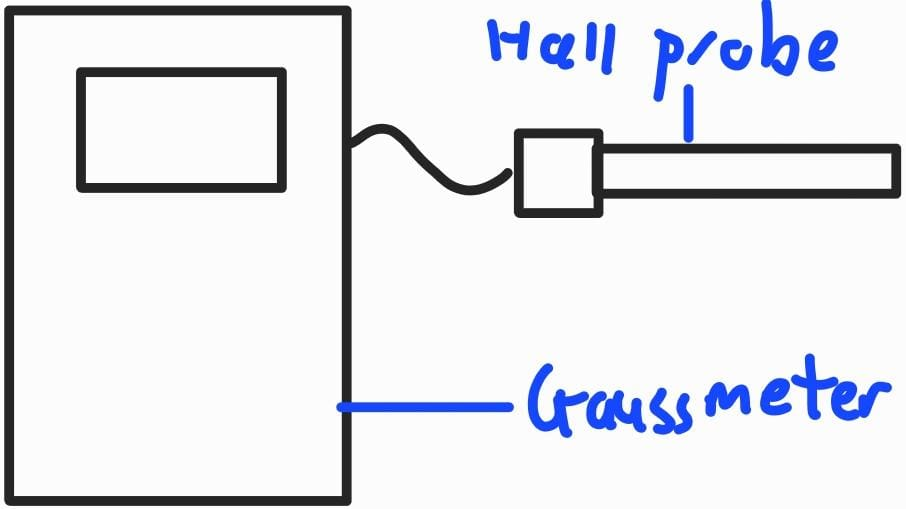
\includegraphics[width=\linewidth]{../images/gaussmeter-Hall-probe.jpg}
    \end{itemize}
    \tabularnewline
    &
    \begin{itemize}
        \item[\(\circ\)] Specify which setting, d.c. or a.c., an ammeter or voltmeter should be used in.
        \item[\(\circ\)] A c.r.o. can either be connected directly to an electrical circuit, or to a microphone. 
        \item[\(\circ\)] A signal generator is an a.c. source with variable frequency, amplitude, and waveform. It can be connected to a loudspeaker.
    \end{itemize}
    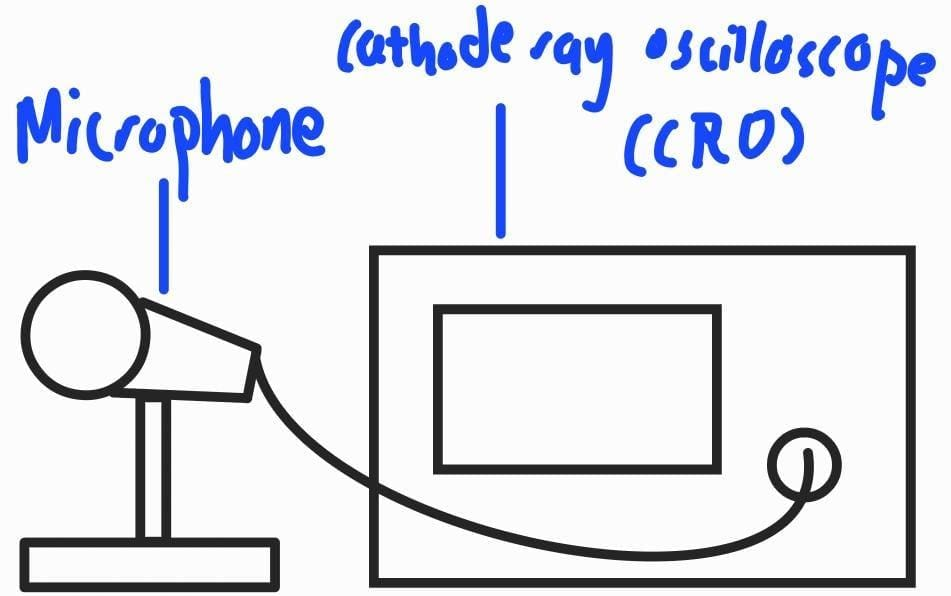
\includegraphics[width=\linewidth]{../images/cro-mic.jpg}
    &
    \begin{minipage}{\linewidth}
        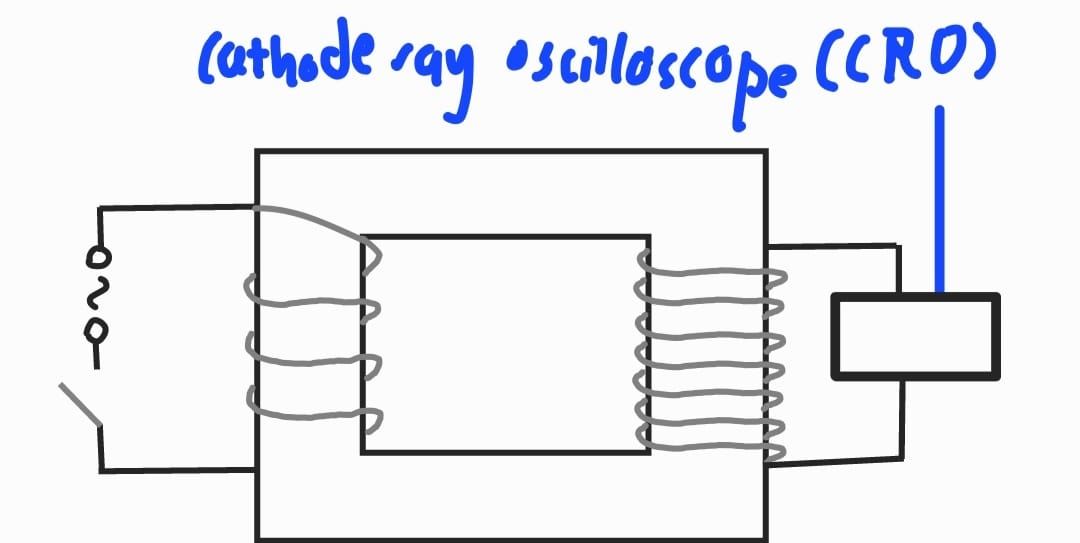
\includegraphics[width=\linewidth]{../images/cro-transformer.jpg}\\
        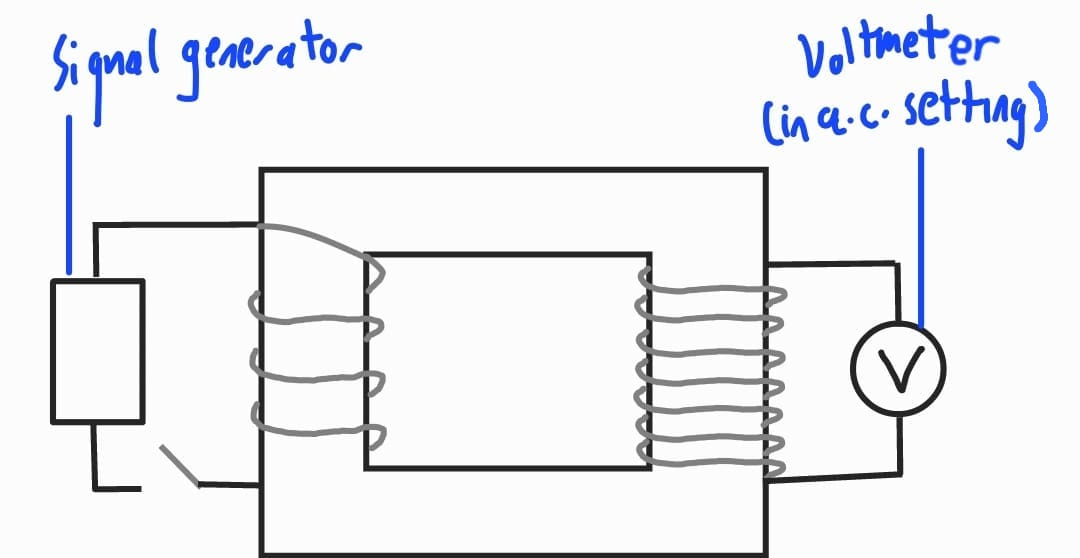
\includegraphics[width=\linewidth]{../images/signal-gen-voltmeter-transformer.jpg}\\
        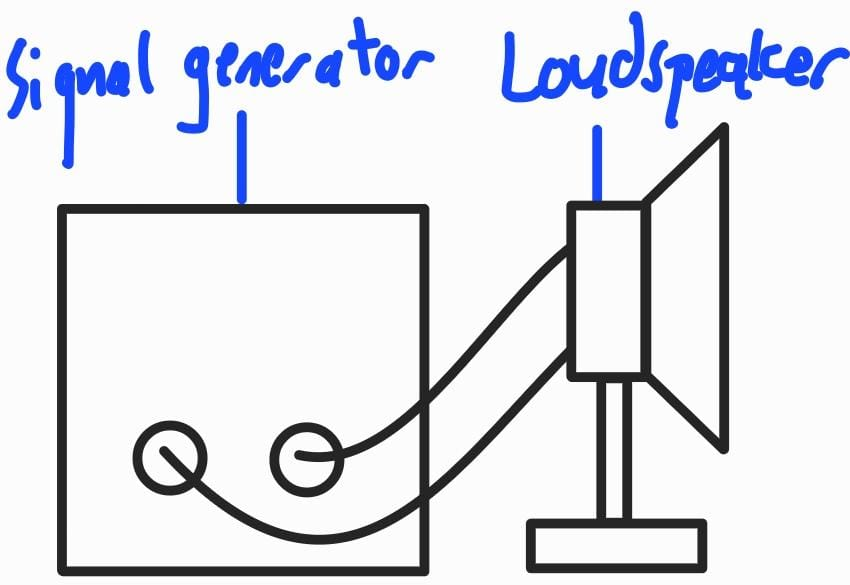
\includegraphics[width=\linewidth]{../images/signal-gen-loudspeaker.jpg}
    \end{minipage}
    \tabularnewline\bottomrule
    \caption{Precautions.}
    \label{table:precautions}
\end{longtable}
\end{document}